\documentclass[11pt]{scrartcl}
\usepackage[sexy]{evan}
\usepackage{graphicx}
\usepackage{float}
\usepackage{pgfplots}
\usepackage{subcaption}
\pgfplotsset{compat=1.18}
\definecolor{dg}{RGB}{2,101,15}
\newtheoremstyle{dotlessP}{}{}{}{}{\color{dg}\bfseries}{}{ }{}
\theoremstyle{dotlessP}
\newtheorem{property}[theorem]{Property}
\newtheoremstyle{dotlessN}{}{}{}{}{\color{teal}\bfseries}{}{ }{}
\theoremstyle{dotlessN}
\newtheorem{notation}[theorem]{Notation}
\newtheoremstyle{dotN}{}{}{}{}{\color{teal}\bfseries}{.}{ }{}
\theoremstyle{dotN}
\newtheorem{solution}{Solution}
\RequirePackage[linesnumbered,lined,boxed,commentsnumbered,noend]{algorithm2e}
\usepackage{algpseudocode}
% Shortcuts
\DeclarePairedDelimiter\ceil{\lceil}{\rceil} % ceil function
\DeclarePairedDelimiter\flr{\lfloor}{\rfloor} % floor function

\DeclarePairedDelimiter\paren{(}{)} % parenthesis

\newcommand{\df}{\displaystyle\frac} % displaystyle fraction
\newcommand{\qeq}{\overset{?}{=}} % questionable equality

\newcommand{\Mod}[1]{\;\mathrm{mod}\; #1} % modulo operator

\newcommand{\comp}{\circ} % composition

% Text Modifiers
\newcommand{\tbf}{\textbf}
\newcommand{\tit}{\textit}

% Sets
\DeclarePairedDelimiter\set{\{}{\}}
\newcommand{\unite}{\cup}
\newcommand{\inter}{\cap}

\newcommand{\reals}{\mathbb{R}} % real numbers: textbook is Z^+ and 0
\newcommand{\ints}{\mathbb{Z}}
\newcommand{\nats}{\mathbb{N}}
\newcommand{\complex}{\mathbb{C}}
\newcommand{\tots}{\mathbb{Q}}

\newcommand{\degree}{^\circ}

% Counting
\newcommand\perm[2][^n]{\prescript{#1\mkern-2.5mu}{}P_{#2}}
\newcommand\comb[2][^n]{\prescript{#1\mkern-0.5mu}{}C_{#2}}

% Relations
\newcommand{\rel}{\mathcal{R}} % relation

\setlength\parindent{0pt}

% Directed Graphs
\usetikzlibrary{arrows}
\usetikzlibrary{positioning,chains,fit,shapes,calc}

% Contradiction
\newcommand{\contradiction}{{\hbox{%
    \setbox0=\hbox{$\mkern-3mu\times\mkern-3mu$}%
    \setbox1=\hbox to0pt{\hss$\times$\hss}%
    \copy0\raisebox{0.5\wd0}{\copy1}\raisebox{-0.5\wd0}{\box1}\box0
}}}

% CS 
% NP
% Modulo without space
\newcommand{\nmod}[1]{\;\mathrm{mod}\;#1}
\newcommand{\np}{\texttt{NP}_\texttt{search}}
\newcommand{\p}{\texttt{P}_\texttt{search}}
\newcommand{\nph}{\texttt{NP}_\texttt{search}\text{-hard}}
\newcommand{\npc}{\texttt{NP}_\texttt{search}\text{-complete}}
\newcommand{\EXP}{\texttt{EXP}_\texttt{search}}
\newcommand{\xxhash}[2]{\rotatebox[origin=c]{#2}{$#1\parallel$}}

\title{CS 124: Data Structures and Algorithms}
\subtitle{Programming Set 3}
\author{Cao and Ziv}
\date{\today}
\newcommand{\courseNumber}{CS 124}
\newcommand{\courseName}{Data Structures and Algorithms}
\newcommand{\psetName}{ProgSet 3}
\newcommand{\dueDate}{Due: Thursday, April 18, 2024}
\newcommand{\name}{Denny Cao and Ossimi Ziv}
\renewcommand{\theques}{\thesection.\alph{ques}} % Change subtheo counter for alpha output
\declaretheorem[style=basehead,name=Answer,sibling=theorem]{ans}
\renewcommand{\theans}{\thesection.\alph{ans}}

% stuff for algorithm environment
%%% Coloring the comment as blue
\newcommand\mycommfont[1]{\footnotesize\ttfamily\textcolor{blue}{#1}}
\SetCommentSty{mycommfont}

\SetKwInput{KwInput}{Input}                % Set the Input
\SetKwInput{KwOutput}{Output}              % set the Output

\makeatletter
\newenvironment{compprob}[1][]
  {\renewcommand{\algorithmcfname}{Computational Problem}%
   \begin{algorithm}[#1]
   \long\def\@caption##1[##2]##3{%
     \par
     \begingroup\@parboxrestore
     \if@minipage\@setminipage\fi
     \normalsize \@makecaption{\AlCapSty{\AlCapFnt\algorithmcfname}}{\ignorespaces ##3}%
     \par\endgroup
   }}
  {\end{algorithm}}
\makeatother
%++++++++++++++++++++++++++++++++++++++++
% title stuff
\makeatletter
\renewcommand{\maketitle}{\bgroup\setlength{\parindent}{0pt}
    \begin{flushleft}
        {\Large\textbf{\@title}} \\ \vskip0.2cm
        \begingroup
            \fontsize{12pt}{12pt}\selectfont
            \courseNumber: \courseName 
        \endgroup \vskip0.3cm
        \dueDate \hfill\rlap{}\textbf{\name} \\ \vskip0.1cm
        \hrulefill
    \end{flushleft}\egroup 
}
\makeatother

\title{\psetName}
\begin{document}
\maketitle
\thispagestyle{plain}
\section{Number Partition}
\begin{compprob}[h]
        \SetKwInOut{Output}{Output~}
        \SetKwInOut{Input}{Input~}
		\Input{A sequence of $n$ numbers $A = \{a_1, a_2, \ldots, a_n\}$}
                        \Output{A sequence of $n$ numbers $S = \{s_1, s_2, \ldots, s_n\}$ of signs $s_i \in \set*{+1,
                            -1}$ such that the residual sum of the numbers in $A$ is minimized.}
                            \caption{Number Partition}
\end{compprob}
\begin{claim}
    \texttt{Number Partition} can be solved in pseudo-polynomial time. 
\end{claim}
\begin{proof}
   Suppose the sequence of terms in $A$ sum up to some number  $b$. Then each of the numbers in  $A$ has at most  $\log
   b$ bits. We will show there exists a dynamic programming algorithm that solves the \texttt{Number Partition} problem
   that takes time polynomial $nb$:
   \begin{itemize}
       \item \textbf{Subproblems:} Let $D[i,j]$ be whether it is possible for  $A[0,i]$ to sum up to $j$.
   
  \item \textbf{Recurrence:} The recurrence relation is given by:
    \[
   D[i,j] = (D[i-1,j+a_i] \lor D[i-1,|j-a_i|])  
   \] 
    Our recurrence is correct because if $D[i-1,j+a_i]$ is true, then we can subtract $a_i$ from $j + a_i$ (which is obtainable with the first $i-1$ elements) to get $j$. 
    Similarly, if $D[i-1,|j-a_i|]$ is true, then either we can add $a_i$ to the $j - a_i$ (which is obtainable with the first $i-1$ elements) to get $j$ or subtract $a_i - j$ (which is obtainable with the first $i-1$ elements) from $a_i$ to get $j$. 
    In doing so, we obtain every
    possible sum of the first $i$ elements of $A$. 

   \item\textbf{Topological Order:} We solve the subproblems in increasing order of $i$ and $j$.

    \item\textbf{Base Case:} $D[0,0] = \texttt{True}$ and $D[i,j] = \texttt{False}$ for all other $i,j$.

    \item\textbf{Original:} The original problem is to find the smallest $j$ such that $D[n,j]$ is true, or:
    \[
    \min \set*{j : D[n,j] == \texttt{True}, j \in [b]}
    \]

   \item \textbf{Time Complexity:} The time complexity of this algorithm is $O(nb)$. This is because for each
    subproblem we check if $b$ sums are possible (The maximum sum is $b$). When checking if a sum is possible, we
    take  $O(1)$ time to check 2 previous subproblems. Thus, the total time complexity is $O(nb)$ to fill the
    table. Iterating to find the smallest $j$ such that $D[n,j]$ is true takes $O(b)$ time. Therefore, the total time
    complexity is $O(nb) + O(b) = O(nb)$.
   \end{itemize}
    Therefore, the \texttt{Number Partition} problem can be solved in pseudo-polynomial time.
\end{proof}

\section{Karmarkar-Karp}
\subsection{Implementation Correctness}
\begin{claim}
Our implementation of \texttt{Karmarkar-Karp} is correct.
\end{claim}
\begin{proof}
     We implement KK by using a python heap-queue as a stand-in for a min-heap. We initialize this min-heap with all the values from A but turned negative. Afterwards, we pop the head twice, and set the popped value to negative. Afterwards we push the negative of the difference of the two elements back onto the heap. We continue this in a loop while the size of the heap is larger than one, when it is just 1, we return that final value.\\

    The correctness of this implementation follows directly from the definition of KK. Our negative value min heap functions as a max-heap, as the largest values will be the smallest negative, and our min-heap correctly has the head as the smallest element. KK instructs we pop the two largest elements and push their difference, which is exactly what we do. In storing the negative of the negative of the largest elements, we are storing the largest elements per requirements. This process will continue until the final differences remains, and we return that value as our residue. So our implementation is correct.    
\end{proof}
\subsection{Runtime}
\begin{claim}
    \texttt{Karmarkar-Karp} can be implemented in $O(n\log n)$ time
\end{claim}
\begin{proof}
    The algorithm suggests that we are given a list of numbers, $A$, we select the two largest elements, $a_i$, and $a_j$, difference them, replace the larger of the two by the absolute value of their difference, and replace the smaller with 0. Repeat this until there is only one number left. To analyze the time complexity of a potential implementation, we can split the problem into steps:
    \begin{itemize}
        \item \textbf{Sorting}: To make it convenient to find the two largest elements, we can create a \texttt{max-heap}. Building this structure will take $O(n)$ time given that $A$ has $n$ elements.
        \item \textbf{Selecting}: Actually extracting the two largest elements involves running \texttt{extract-max} twice from our max-heap. Each of these extractions and restructuring of the heap afterwards will take $O(\log n)$ time.
        \item \textbf{Comparison}: Comparing the two values and computing their difference involves basic arithmetic and can be done in constant time given the problem definition. 
        \item \textbf{Inserting}: Inserting both the absolute value of the difference back into the heap takes $O(\log n)$ time. 
    \end{itemize}
    Every time we replace one of the elements with zeros, we are one step closer to the algorithm terminating, going from $n$ steps left to 1 step left. (given that it ends when the two max's are a number and zero). So the number of iterations of the [select, compare, insert loop] that we have to do is $n-1$. As a result, our time complexity is $O(n * (\log n + 1 + 1)) + O(n) = O(n\log n + n) + O(n) = O(n\log n)$.\\

    Therefore we have shown it is possible to implement the Karmarkar-Karp algorithm in $O(n \log n)$.
\end{proof}
\section{Experimental Data}
\subsection{Residue Results}
We run each algorithm on 50 random inputs of size 100 of numbers between 1 and $10^{12}$. The following table lists the obtained residues and the bottom provides statistics regarding the distribution of the data.
\begin{table}[H]
   \centering
   \resizebox{\textwidth}{!}{%
\begin{tabular}{c|c|c|c|c|c|c|c}
Trial         & KK          & Repeated Random & Hill Climbing & Simulated Annealing & Repeated Random PP & Hill Climbing PP & Simulated Annealing PP \\
\hline
1             & 244473      & 87970267        & 479660689     & 617418391           & 139                & 809              & 619                    \\
2             & 84884       & 388599116       & 64090022      & 26767974            & 206                & 100              & 366                    \\
3             & 258684      & 346452394       & 266278248     & 420919554           & 164                & 384              & 396                    \\
4             & 6174        & 167827416       & 474556064     & 120672690           & 138                & 300              & 488                    \\
5             & 483295      & 64315015        & 19701433      & 177241003           & 25                 & 1331             & 395                    \\
6             & 40663       & 155202693       & 78025915      & 867005015           & 237                & 1149             & 375                    \\
7             & 168632      & 116734588       & 65383618      & 119895416           & 340                & 172              & 190                    \\
8             & 51501       & 56079063        & 447848611     & 86428589            & 159                & 511              & 81                     \\
9             & 775712      & 100676834       & 73848338      & 276347990           & 112                & 764              & 266                    \\
10            & 171145      & 136885643       & 623360859     & 415262813           & 61                 & 341              & 11                     \\
11            & 58008       & 393328788       & 37014528      & 19382122            & 434                & 1224             & 150                    \\
12            & 24280       & 361491808       & 484961426     & 205644234           & 368                & 148              & 92                     \\
13            & 10974       & 49271278        & 302736382     & 245593308           & 82                 & 1002             & 410                    \\
14            & 172136      & 207342100       & 470097020     & 60624376            & 126                & 86               & 486                    \\
15            & 3585        & 340416893       & 116651015     & 14812321            & 159                & 275              & 47                     \\
16            & 33432       & 865642540       & 410532980     & 160613914           & 126                & 622              & 1096                   \\
17            & 143         & 329411          & 967433737     & 372864795           & 201                & 163              & 221                    \\
18            & 962140      & 181581092       & 261866056     & 127447726           & 490                & 722              & 80                     \\
19            & 554006      & 117974366       & 1240920932    & 178452762           & 24                 & 376              & 2                      \\
20            & 112412      & 6489336         & 794041684     & 2783760             & 56                 & 234              & 34                     \\
21            & 170727      & 237001175       & 225618415     & 389633141           & 299                & 1487             & 313                    \\
22            & 279936      & 28828900        & 309463910     & 41130106            & 402                & 498              & 918                    \\
23            & 296606      & 26365600        & 16537204      & 551501002           & 284                & 2744             & 204                    \\
24            & 27017       & 175579403       & 192076169     & 1046123043          & 291                & 347              & 89                     \\
25            & 113370      & 328204226       & 32709020      & 94885590            & 104                & 552              & 4                      \\
26            & 244482      & 391954306       & 182539024     & 114982318           & 338                & 282              & 196                    \\
27            & 80211       & 352541825       & 11880739      & 583763855           & 59                 & 339              & 1053                   \\
28            & 970955      & 287546935       & 186366763     & 61247253            & 17                 & 115              & 317                    \\
29            & 38954       & 152866070       & 1183412312    & 72222452            & 76                 & 114              & 1600                   \\
30            & 62896       & 1442073504      & 26836576      & 335548102           & 106                & 474              & 72                     \\
31            & 78064       & 116357704       & 316750910     & 74219914            & 46                 & 486              & 42                     \\
32            & 247097      & 112957413       & 103576333     & 95842399            & 327                & 637              & 9                      \\
33            & 28387       & 440802925       & 232817921     & 108422899           & 291                & 811              & 171                    \\
34            & 82046       & 49821758        & 932563088     & 517656356           & 230                & 150              & 520                    \\
35            & 889934      & 122909990       & 16343172      & 6650736             & 180                & 410              & 292                    \\
36            & 431656      & 116959242       & 169087112     & 172472186           & 132                & 1004             & 154                    \\
37            & 89536       & 883338848       & 383142950     & 71602650            & 80                 & 1578             & 306                    \\
38            & 5762        & 120802670       & 10515672      & 535112268           & 174                & 594              & 38                     \\
39            & 28200       & 24722356        & 92789004      & 47446672            & 18                 & 288              & 40                     \\
40            & 84184       & 973345298       & 103593130     & 375220032           & 192                & 386              & 178                    \\
41            & 1108778     & 588007418       & 248459030     & 386999234           & 200                & 538              & 88                     \\
42            & 766812      & 515115316       & 35200062      & 382247548           & 12                 & 80               & 190                    \\
43            & 29498       & 695616536       & 40575632      & 118055214           & 372                & 174              & 388                    \\
44            & 327435      & 295223941       & 885184889     & 51363879            & 181                & 17               & 95                     \\
45            & 778858      & 534048582       & 316890746     & 133753228           & 136                & 158              & 114                    \\
46            & 144740      & 383922936       & 343537194     & 96599956            & 16                 & 188              & 126                    \\
47            & 101282      & 401792774       & 7321098       & 495829530           & 64                 & 92               & 18                     \\
48            & 20738       & 273147518       & 176867886     & 67728960            & 398                & 492              & 500                    \\
49            & 249682      & 613769208       & 150446866     & 326700622           & 300                & 1250             & 412                    \\
50            & 202743      & 863633311       & 28468689      & 476212423           & 83                 & 215              & 155                    \\
\hline
Mean          & 243937.30   & 313877366.58    & 292811621.46  & 246947046.42        & 181.10             & 544.26           & 288.14                 \\
Min           & 143         & 329411          & 7321098       & 2783760             & 12                 & 17               & 2                      \\
Max           & 1108778     & 1442073504      & 1240920932    & 1046123043          & 490                & 2744             & 1600                   \\
Std Deviation & 296087.0937 & 297119884.2     & 311699136.2   & 231103092.6         & 125.799849         & 506.885319       & 315.726245             \\
25\%          & 39381.25    & 116451925       & 64413421      & 72721817.5          & 80.5               & 177.5            & 82.75                  \\
50\%          & 112891      & 222171637.5     & 189221466     & 147183571           & 159                & 385              & 190                    \\
75\%          & 274623      & 392985167.5     & 403685472.5   & 385811312.5         & 289.25             & 700.75           & 393.25                
\end{tabular}}
\caption{Experimental Data}
\end{table}
\begin{figure}[H]
   \centering 
   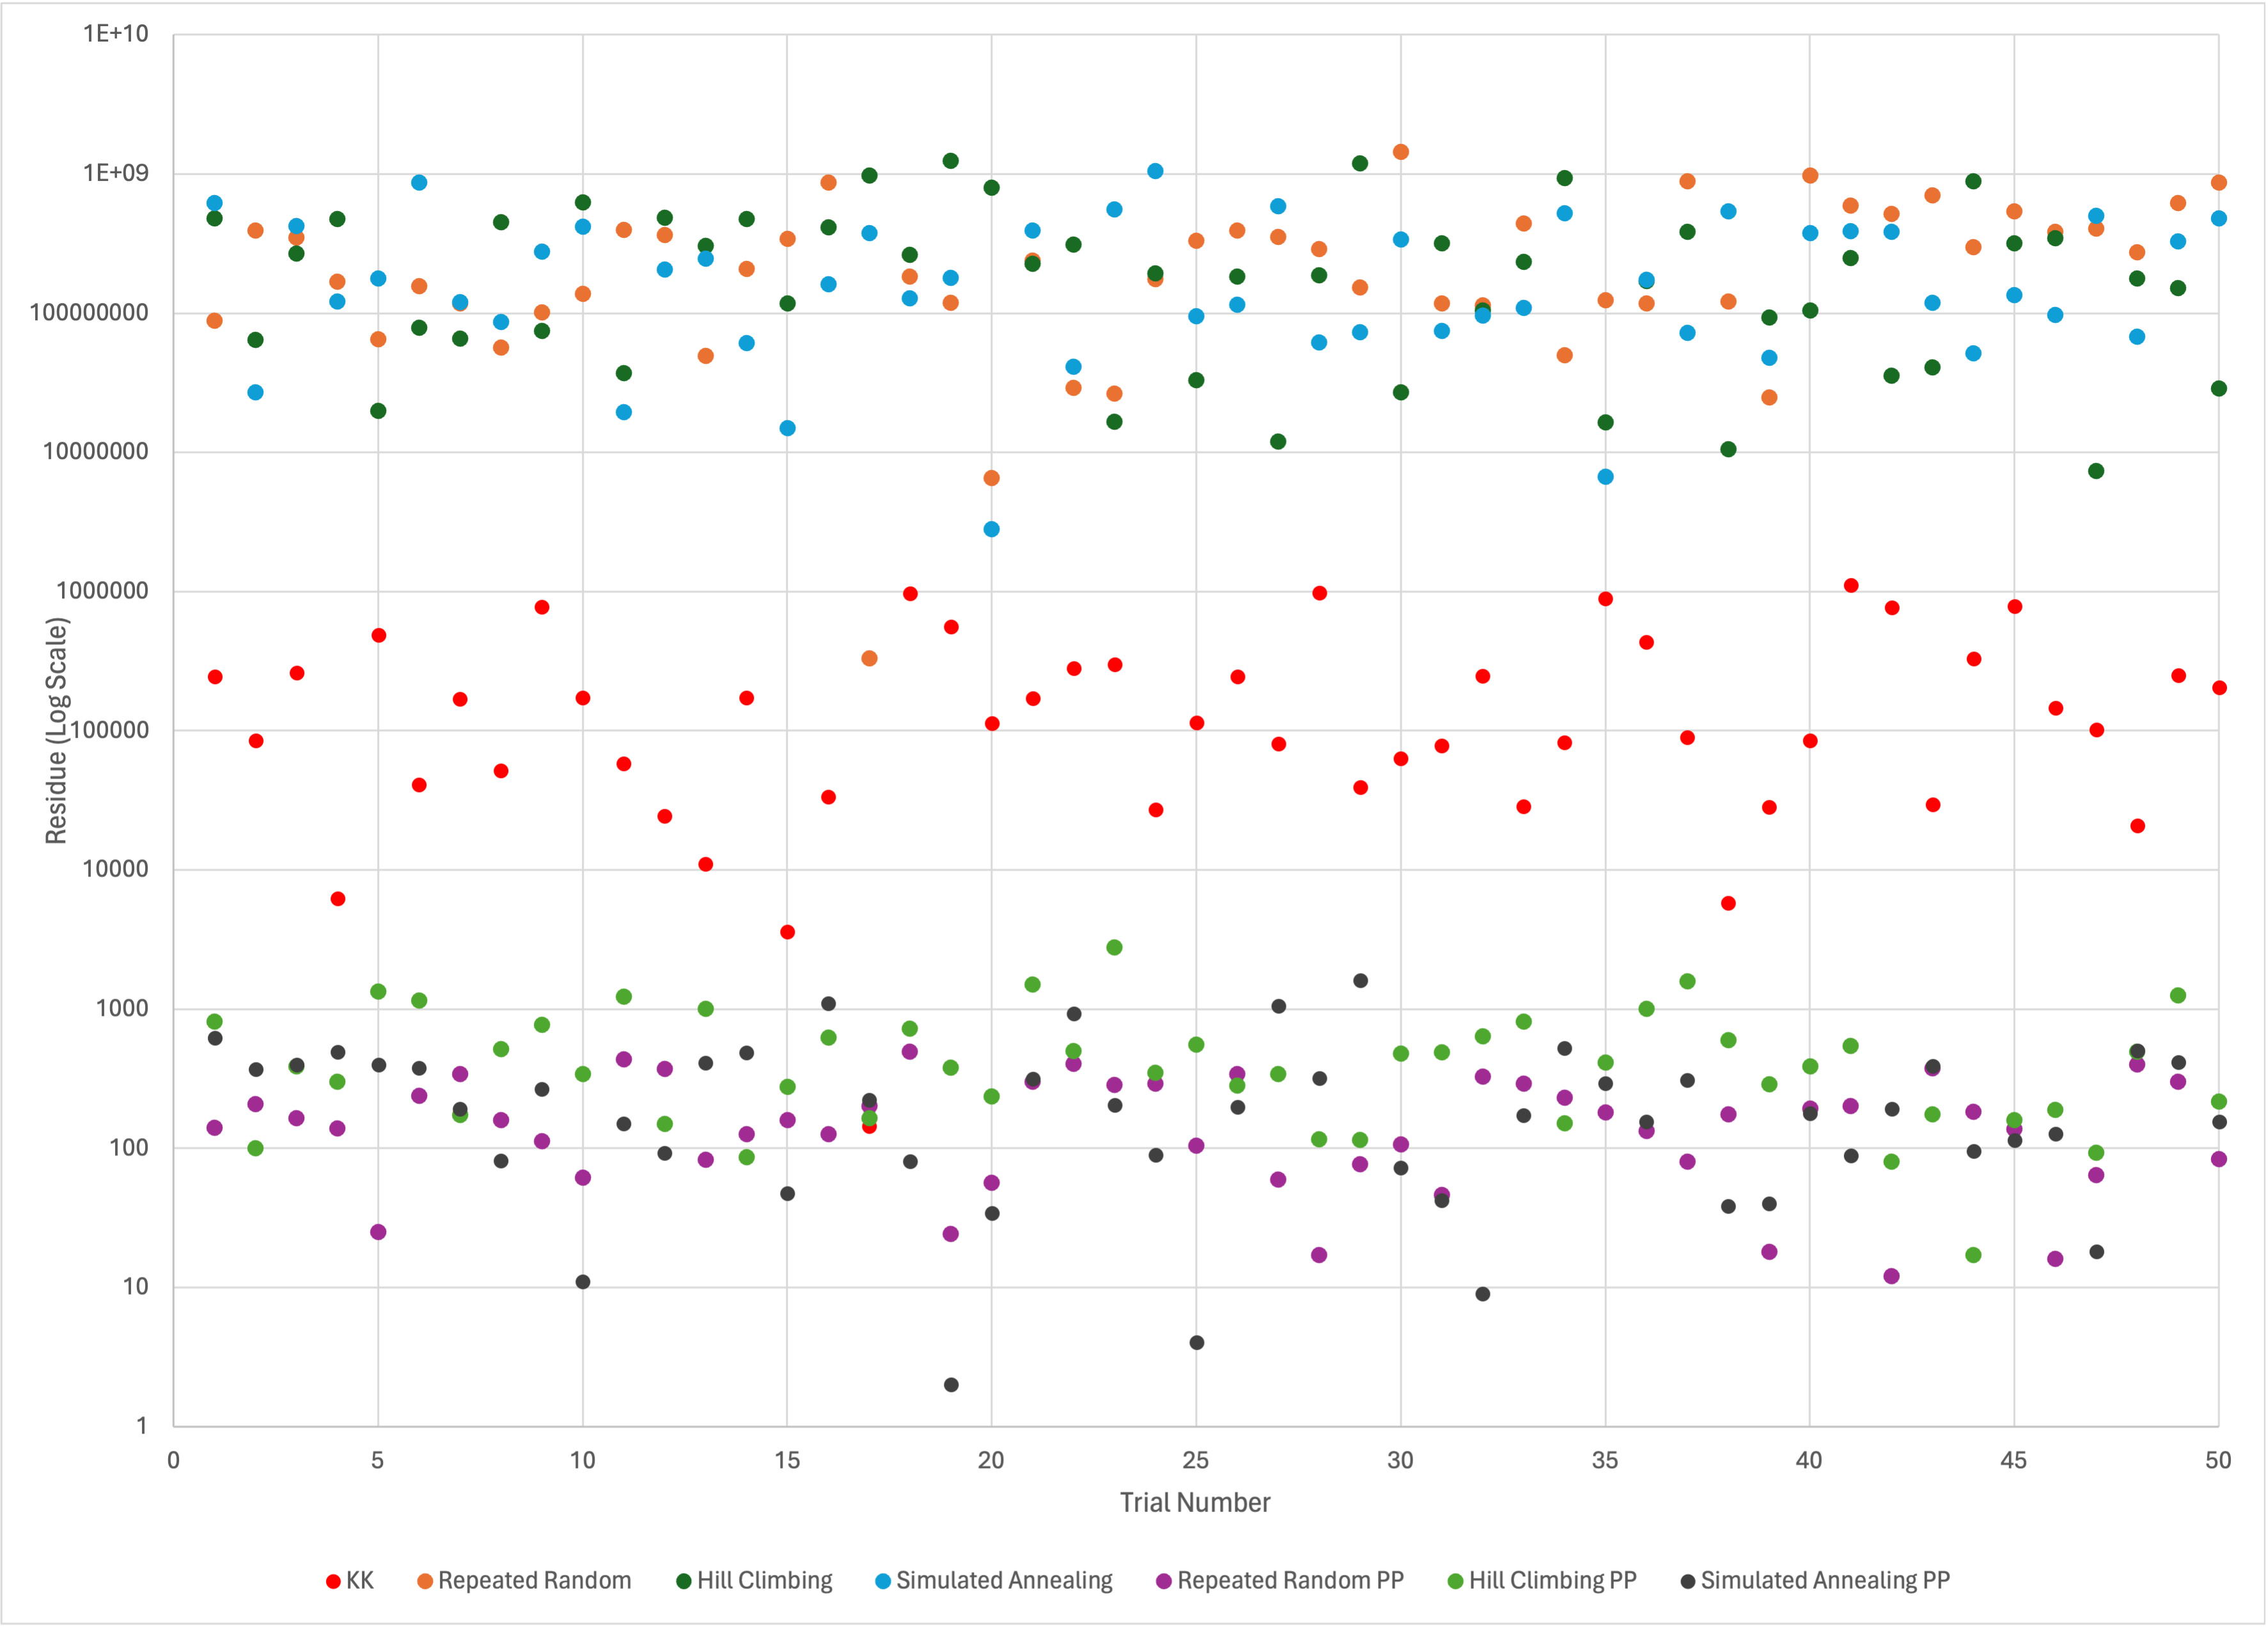
\includegraphics[width=\textwidth]{Picture1.png}
   \end{figure}
\subsection{Timing}
\begin{table}[H]
   \centering 
   \resizebox{\textwidth}{!}{%
\begin{tabular}{c|c|c|c|c|c|c|c}
Trial & KK        & Repeated Random & Hill Climbing & Simulated Annealing & Repeated Random PP & Hill Climbing PP & Simulated Annealing PP \\
\hline
1     & 5.29E-05  & 0.17540407      & 0.07839704    & 0.13006902          & 2.28987408         & 2.21262527       & 3.347615               \\
2     & 3.93E-05  & 0.17427373      & 0.07609701    & 0.12669206          & 2.29126692         & 2.35132694       & 3.38014102             \\
3     & 3.89E-05  & 0.17631197      & 0.07664824    & 0.12858868          & 2.28913736         & 2.51783299       & 3.69098592             \\
4     & 4.41E-05  & 0.17306495      & 0.07654309    & 0.12646294          & 2.30573201         & 2.17773008       & 3.34503436             \\
5     & 3.81E-05  & 0.17174292      & 0.07670498    & 0.12639809          & 2.3586812          & 2.14093184       & 3.3778429              \\
6     & 3.67E-05  & 0.17232108      & 0.07682395    & 0.12759781          & 2.27806211         & 2.18601823       & 3.68913484             \\
7     & 3.70E-05  & 0.17067599      & 0.07574797    & 0.12511396          & 2.30559301         & 2.21349382       & 3.41671705             \\
8     & 4.03E-05  & 0.17109489      & 0.076612      & 0.12643695          & 2.33348298         & 2.30946302       & 3.42526102             \\
9     & 4.20E-05  & 0.17145491      & 0.07709503    & 0.12631178          & 2.32563829         & 2.35571694       & 3.43559384             \\
10    & 4.60E-05  & 0.16894388      & 0.07536793    & 0.1242702           & 2.28250694         & 2.33226371       & 3.65103698             \\
11    & 3.70E-05  & 0.16936684      & 0.07628918    & 0.125453            & 2.30748296         & 2.29763293       & 3.42228818             \\
12    & 3.72E-05  & 0.17246294      & 0.07819104    & 0.12659597          & 2.26848793         & 2.13310814       & 3.41908193             \\
13    & 3.70E-05  & 0.16926575      & 0.07616615    & 0.12893987          & 2.3469131          & 2.20960689       & 3.40671635             \\
14    & 3.62E-05  & 0.17219377      & 0.0782702     & 0.13370776          & 2.3095212          & 2.23313475       & 3.58830214             \\
15    & 3.79E-05  & 0.17466617      & 0.07780695    & 0.12521815          & 2.31600213         & 2.20623899       & 3.43248391             \\
16    & 4.29E-05  & 0.16876602      & 0.07674217    & 0.12565875          & 2.33569789         & 2.26488996       & 3.42939615             \\
17    & 3.60E-05  & 0.16964293      & 0.0780921     & 0.12467909          & 2.37793612         & 2.46837783       & 3.64588094             \\
18    & 4.91E-05  & 0.18189812      & 0.07779098    & 0.12800097          & 2.300565           & 2.42687583       & 3.41397309             \\
19    & 3.89E-05  & 0.17286301      & 0.07741523    & 0.12814164          & 2.35048127         & 2.25900507       & 3.51661491             \\
20    & 4.20E-05  & 0.17370105      & 0.077564      & 0.12845588          & 2.29587722         & 2.23238778       & 3.41408515             \\
21    & 3.91E-05  & 0.17202902      & 0.07681012    & 0.12824488          & 2.3612771          & 2.22989678       & 3.41864705             \\
22    & 4.01E-05  & 0.17349887      & 0.07902527    & 0.12722683          & 2.32172608         & 2.28568792       & 3.61887002             \\
23    & 3.89E-05  & 0.17483902      & 0.07818794    & 0.12813807          & 2.34055805         & 2.29791212       & 3.49329782             \\
24    & 4.39E-05  & 0.17300105      & 0.07726002    & 0.12870598          & 2.30363488         & 2.24057078       & 3.51497793             \\
25    & 4.58E-05  & 0.17140126      & 0.07860303    & 0.12996578          & 2.31218934         & 2.29513168       & 3.43592191             \\
26    & 3.81E-05  & 0.17419171      & 0.07731628    & 0.12783003          & 2.30007291         & 2.24052501       & 3.57271791             \\
27    & 3.72E-05  & 0.1741581       & 0.07769608    & 0.12801909          & 2.36652088         & 2.34660006       & 3.51849699             \\
28    & 3.81E-05  & 0.17570114      & 0.07828522    & 0.13051009          & 2.41483092         & 2.38253498       & 3.49378514             \\
29    & 3.70E-05  & 0.17596292      & 0.07783604    & 0.12846327          & 2.3593688          & 2.41654706       & 3.4488802              \\
30    & 4.03E-05  & 0.17640185      & 0.07856321    & 0.12936497          & 2.3164928          & 2.36144209       & 3.44335413             \\
31    & 3.81E-05  & 0.17440391      & 0.07901907    & 0.12957406          & 2.35207391         & 2.23148489       & 3.648772               \\
32    & 3.72E-05  & 0.17465901      & 0.07751989    & 0.12820816          & 2.30580187         & 2.28986406       & 3.46296                \\
33    & 3.79E-05  & 0.17542815      & 0.07750392    & 0.13928699          & 2.31818175         & 2.24462414       & 3.49628091             \\
34    & 3.79E-05  & 0.17551398      & 0.07751083    & 0.12947726          & 2.33022594         & 2.29789996       & 3.46237397             \\
35    & 4.79E-05  & 0.17393112      & 0.07775784    & 0.12674403          & 2.34067893         & 2.27311087       & 3.65385008             \\
36    & 3.91E-05  & 0.17436695      & 0.07797503    & 0.12988281          & 2.34572411         & 2.38500476       & 3.48577499             \\
37    & 4.72E-05  & 0.17605805      & 0.07854819    & 0.12885594          & 2.32972217         & 2.24011087       & 3.43393517             \\
38    & 3.70E-05  & 0.17748594      & 0.0775671     & 0.12820387          & 2.38292694         & 2.27854991       & 3.43331003             \\
39    & 3.91E-05  & 0.17555809      & 0.0783968     & 0.12812901          & 2.34181404         & 2.29153085       & 3.55212402             \\
40    & 3.91E-05  & 0.17554688      & 0.0777328     & 0.12854385          & 2.32558513         & 2.37445211       & 3.62642884             \\
41    & 3.89E-05  & 0.17428303      & 0.078022      & 0.12878609          & 2.37403584         & 2.32890224       & 3.4269309              \\
42    & 3.72E-05  & 0.17356491      & 0.07738686    & 0.12879014          & 2.34025502         & 2.18840003       & 3.53366876             \\
43    & 3.89E-05  & 0.17490602      & 0.07949018    & 0.13073897          & 2.32471585         & 2.39597297       & 3.67679119             \\
44    & 3.79E-05  & 0.1757412       & 0.07915974    & 0.1300211           & 2.35176897         & 2.2420032        & 3.45233774             \\
45    & 3.79E-05  & 0.17412138      & 0.07721972    & 0.12782097          & 2.35584211         & 2.24205089       & 3.454391               \\
46    & 3.89E-05  & 0.1731441       & 0.07721186    & 0.1277833           & 2.35742378         & 2.35651994       & 3.5206573              \\
47    & 4.03E-05  & 0.17622185      & 0.07761312    & 0.12767792          & 2.32881999         & 2.48536611       & 3.81021714             \\
48    & 4.60E-05  & 0.17662787      & 0.07871103    & 0.129246            & 2.35728216         & 2.33584094       & 3.41722393             \\
49    & 4.01E-05  & 0.17489409      & 0.07787681    & 0.12824512          & 2.38670683         & 2.31936407       & 3.52481675             \\
50    & 4.12E-05  & 0.17890692      & 0.07933378    & 0.13204503          & 2.35906982         & 2.34447622       & 3.47601008             \\
\hline
Mean  & 0.0000401 & 0.1739333       & 0.0776301     & 0.1283464           & 2.3314853          & 2.2954208        & 3.4991198             
\end{tabular}}
\caption{Time Data for Each Trial}
\end{table}
\section{Discussion}
When plotted as a scatter plot using a log scale for the $y$-axis, we begin to see ``striations'' of algorithms using standard interpretation for a solution, using Karmarkar-Karp, and algorithms using prepartition interpretation for a solution. Karmarkar-Karp throughout all trials is bounded above by residues obtained through standard solution algorithms and bounded below by residues obtained through prepartition solution algorithms.
\\

The most significant difference between standard algorithms and prepartition algorithms lies within the initial random solution. We observe this through the behavior of Repeated Random for both standard and prepartition interpretations. Repeated Random improves upon the initial random solution by generating a new random solution and replacing if the residue is less. We can conclude that, on average, the standard solution will produce a worse solution as with even the best random solution out of 25,000 iterations, of around 3 orders of magnitude greater residue for the standard algorithm. 
\\

We also observe that the neighbors of the random solution does not matter a significant amount through how close the result of Hill Climb and Simulated Annealing for both standard and prepartition interpretations are to the Repeated Random residues, where Hill Climb shows that picking better neighbors each time will not yield a significant improvement, and walking to random neighbors to avoid local minimums does not either.
\\

In terms of run time, Karmarkar-Kar is the fastest of all the algorithms and prepartition algorithms are the slowest. This makes sense as the prepartition algorithms call Karmarkar-Kar in order to obtain the residue of neighbors/random solutions 25,000 times (The amount we set \texttt{max\_iter}). 
\\

Hill Climbing algorithms are the fastest for both interpretations, with Repeated Random being the slowest for standard solution algorithms and Simulated Annealing being the slowest for prepartiion algorithms.

From the results, it is evident that KK is a much more efficient algorithm than the random selectors, having a median three orders of magnitude lower. It's noteworthy that the mean is triple the median for KK, and observing the graph we see that the variance is very large, with the spread going from ~2000 to ~5,000,000. This variance and sparsity among the points is significantly emphasized in KK.\\

Among the three randomized algorithms, All through roughly had the same mean but simulated annealing had a considerably better median. This can be observed on the graph as a significant portion of its data points are spread lower than the other two.\\

It is also evident that results get exponentially better when we pre-partition. By doing so and moving away from totally random solutions, we can see that we consistently get far smaller values. The results are also orders of magnitude better than KK, demonstrating the merit of arbitrary group selecting and not a binary sign assignment.



\section{Using Karmarkar-Karp as a starting point}
\subsection{Algorithmic Improvements}
Using KK as a starting point for the standard random algorithms (not prepartitioned) we'd expect to get varying levels of improvement depending on the algorithm, and we can verify these expectations empirically.
\begin{itemize}
    \item \textbf{Repeated Random}: Using the starting point from KK in the repeated random algorithm will provide a strong lower bound for the quality of the solution generated. Any random improvement will further the quality of this bound. The random nature of the algorithm would be equally likely to \textit{improve} on this regardless of the starting point, but as we can observe empirically by comparing the performance of the two algorithms, merely feeding in the KK solution as a baseline will greatly increase the quality of the random result.
    \item  \textbf{Hill Climbing}: This case is relatively similar to the previous. Setting KK as our starting point in Hill Climbing will definitely allow us to refine the solution further per the nature of the hill climbing algorithm selecting the best possible neighbor. That said, it couuld potentially trap us in a local minimum residue that isn't the global minimum. Even still, already having a strong starting point will provide a good jumping off point and any improvement will be even closer to ideal as opposed to starting in a random assortment. We can again observe empirically that KK far surpasses hill climbing in quality given the latter's random start. 
    \item \textbf{Simulated Annealing}: Again given the already strong solution from KK, the exploration involved in not picking an always better neighbor will allow for ideal use of this jumping off point. The original random starting point has a good chance to be too far away to explore ideal possibilities fully before temperature allows exploration. With KK's decent residue, conditions are well suited for the simulated annealing to explore neighboring solutions and quickly approach the a good minimum residue. Empirical results support that KK is more efficient than simulated annealing and thus its starting point would benefit the algorithms performance. 
    \item \textbf{Effect on Prepartition}: Using KK to start for the prepartition will create a binary assignment to two sign groups among which the elements will be split. This is in essence the same as creating a $P$ array such that the numbers are all $1$ or $2$. Consequently, the selection of neighbors will vary than if we had pre-partitioned normally where the group assignment is variable $1...N$. The swaps would be between two selected sets of elements as opposed to the potential to affect multiple groups. This would limit exploration and be worse than normal pre-partitioning given the fixed sets created by KK limiting move freedom.\\

    Empirically, this is supported, given that all the prepartitioned random algorithms performed significantly better than KK. 
    \subsection{Runtime Improvements}
    There's no reason to believe given our implementation and data that KK as a starting point would affect runtime in anyway. The algorithms' loops only terminate when a counter reaches max-iter, thus, given that we do not have any conditions to terminate otherwise, a different starting point will not change this algorithm iterating through its entire loop. 
\end{itemize}
\end{document}
